\chapter{Implementación}

En este capítulo se exponen ciertas explicaciones relacionadas con el desarrollo del frontend (implementación de la aplicación web) y el backend (implementación del nuevo servicio en Helpnex).

\section{Implementación del frontend}

El frontend de la aplicación web se realiza con React utilizando los lenguajes de programación \textit{javascript}, \textit{HTML}, y \textit{CSS}.\\

Para la comunicación del frontend con el backend mediante WebSockets se utiliza la librería \textit{reconnecting-websocket} \cite{reconect-ws}. Se decide utilizar esta frente a otras porque reconecta automáticamente con el servicio si la conexión se cierra por alguna razón y es compatible con \textit{WebSocket Browser API} \cite{api-ws-front}. \\


% Explicar que se recibe directamente la información a mostrar, qué es lo que se trata o no (por ejemplo el ordenar por actual que se realiza en el frontend, el filtrado por plantas, el procesado para el mapeado por habitaciones y prioridad).
La aplicación web es una aplicación visual, en la que no se puede realizar ninguna acción sobre las alertas. Se recibe por websockets toda la información necesaria a monitorizar que procesa el nuevo servicio implementado en PAServidor. Por esta razón, la mayoría de la implementación de esta parte del proyecto se centra en interfaz de usuario aunque también se realiza el tratado de la información que llega para tener los datos de la manera indicada. Cabe destacar que el filtrado por plantas de las alertas, la ordenación de las alertas por más actuales, el filtrado de alertas por prioridad y el mapeado por habitaciones, se realiza en esta parte del proyecto.\\


% Indicar otras librerías utilizadas en el proyecto
Para implementar la aplicación web se ha considerado útil contar con el apoyo de ciertas librerías. Algunas interesantes de mencionar son:
\begin{itemize}
	\item \textit{Bootstrap} \cite{bootstrap} y \textit{React-Bootstrap} \cite{react-bootstrap} como herramientas para la implementación de la interfaz de usuario.
	\item \textit{react-multi-carousel} \cite{react-multi-carousel} para mostrar el carrusel de alertas en una de las pantallas principales de la aplicación.
	\item \textit{react-icons} \cite{react-icons} ya que provee distintos tipos de iconos para la aplicación.
	\item \textit{react-moment} \cite{react-moment} como apoyo para utilizar las fechas y horas de las alertas y ordenarlas para mostrar en el carrusel las más actuales primero.
	\item \textit{react-img-mapper} \cite{react-img-mapper} para facilitar el mapeado de las áreas de las habitaciones en los planos de las plantas y poder mostrar al usuario las habitaciones coloreadas por prioridad junto con el icono de la alerta con más prioridad dentro de dicha habitación y la tarjeta emergente con la información de dicha alerta.
\end{itemize}

 % Explicar organización de ficheros en frontend indicando que cierta división de los módulos hace que la organización del código queda bien repartida teniendo las funcionalidades para poder ver a simple vista implementado

Durante el desarrollo de la aplicación se ha seguido cierta estructura a la hora de dividir los módulos para organizar el código. De esta forma, ha sido más fácil realizar una implementación clara durante el desarrollo. Además, de cara a que la empresa pueda reutilizar el código hace que sea más sencillo comprenderlo. Se puede ver la organización realizada  en tiempo de desarrollo con una vista de módulos en forma de diagrama de paquetes. (Véase la Figura 3.1).\\

\begin{figure}[H]
    \centering
    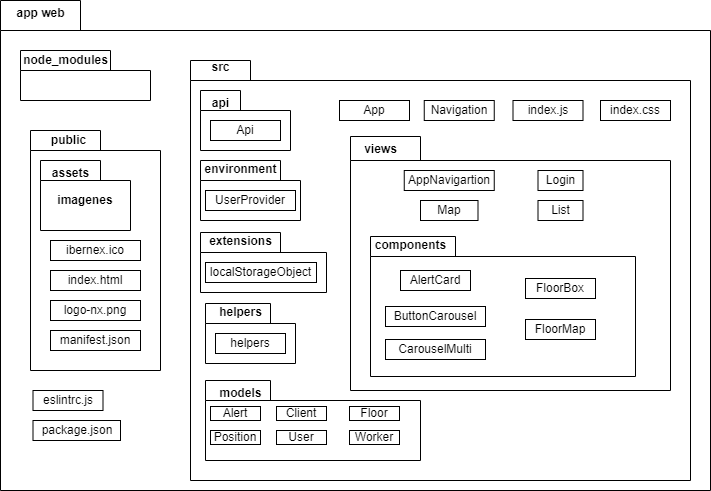
\includegraphics[width=12cm]{Imagenes/Diagrama-paquetes-frontend}
    \caption{Diagrama de paquetes frontend}
    \label{fig:paquetes-frontend}
\end{figure}


En el diagrama se pueden ver distintos paquetes que cumplen distintas funcionalidades. Se explican a continuación:

\textbf{app web} contiene \textit{package.json} que es un archivo de metadatos que contiene información sobre el proyecto como las dependencias; \textbf{node\_modules} que contiene todos los paquetes y dependencias de npm que se especifican en el archivo anterior; y \textit{eslintrc.json} que es el archivo de configuración para ESLint y que se ha utilizado para tener un código limpio y libre de errores. Por otro lado, se tienen los paquetes:
\begin{itemize}
	\item \textbf{public} que contiene archivos estáticos para el navegador. \textit{assets} contiene imágenes para la aplicación; \textit{manifest.json} y \textit{index.html} que son archivos de configuración de la página web; y otros iconos como el utilizado como favicon.
	\item \textbf{src} Contiene distintos modulos esenciales que son el punto de entrada de la aplicación, la navegación y la configuración de ciertos estilos de la aplicación. Además, se puede ver la organización escogida a la hora de implementar la aplicación con la explicación de la funcionalidad de los paquetes que contiene:
	\begin{enumerate}
		\item \textbf{api}: módulo relacionado con la conexión con el backend.
		\item \textbf{environment} y \textbf{localstorageObject}: módulos que gestionan y proporcionan información del usuario en todo el contexto de la aplicación.
		\item \textbf{models}: módulo que contiene los distintos modelos de datos utilizados en la aplicación web.
		\item \textbf{views}: módulo que contiene las vistas principales de la aplicación y \textbf{components} que contiene distintos módulos utilizados por dichas vistas.
		\item \textbf{helpers}: módulo que contiene un módulo que es utilizado por los módulos de views y que contiene funciones auxiliares.
	\end{enumerate}
\end{itemize}


Otra de las decisiones tomadas en la implementación es utilizar en el login la validación del formulario de bootstrap. De esta forma, los datos no se envían a backend a no ser que todos los campos estén completados. Además, en backend se hace la validación correspondiente, y si hay algún problema se informa al usuario de dicho problema mediante una tarjeta emergente. (Se puede ver un ejemplo en la \hyperref[fig:login-error]{Figura E.1} del \hyperref[anexo-e]{Anexo E}).\\

Como se explicará en la siguiente sección, el frontend tiene la información de los clientes y trabajadores desde el inicio de sesión, y cuando le llega información de nuevas alertas debe completar cierta información con la que ya tiene. Por esta razón, para que sea rápido y eficiente, se decide guardar esta información en diccionarios para un fácil y rápido acceso al dato concreto a utilizar. 

\newpage
\section{Implementación del backend}

El backend de la aplicación se realiza con \textit{.NET Framework 4.8}, ya que como se ha explicado en secciones anteriores la implementación que se realiza es concretamente añadir funcionalidad a la aplicación existente. \\

Para la comunicación con el frontend mediante WebSockets se utiliza la librería \textit{websocket-sharp} \cite{websocket-sharp} en su versión \textit{1.0.3.0}.
Se decide utilizar esta librería ya que en otra de las funcionalidades existente en la aplicación se utiliza (aunque en una versión anterior), y se cree conveniente utilizar algo similar de cara a que internamente en la empresa puedan entender mejor la implementación o reutilizar el código.
La instalación de esta librería se realiza mediante el propio Visual Studio (que se ha comentado la sección de herramientras de trabajo que es el entorno de desarrollo utilizado para implementar el backend) utilizando la opción de administrar paquetes NuGet e instalando el nombrado. \\

Al principio la empresa propuso realizar la comunicación del backend con el frontend utilizando \textit{SignalR} \cite{signalr} pero finalmente se descarta por incompatibilidad con la aplicación actual y simplicidad en la arquitectura software. Se puede ver más información referente a esta decisión en el \hyperref[anexo-b]{Anexo B}. \\


% Explicar qué SERVICIO implemento dentro de la arquitectura
De los servicios y eventos nombrados en la arquitectura detallada del PAServidor en la \hyperref[section-arquitectura]{sección 2.2}, el servicio que se ha implementado para añadir funcionalidad a la aplicación existente y que sirve como backend de la aplicación web, es el \textit{Servicio de monitorización web} que se puede observar en la sección nombrada, concretamente en la \hyperref[fig:PAServidor]{Figura 2.2}.\\

%Explicar decisiones tomadas en la implementación del servicio
Durante la implementación del servicio se han tomado distintas decisiones. Algunas de ellas se exponen a continuación.\\

% - Carga de datos iniciales en vez de acceso siempre a base de datos
Cuando un usuario inicia sesión en la aplicación web se envía una carga de datos iniciales con la información acerca de la configuración del centro (plantas con su información y sus planos), los clientes, los trabajadores, y las alertas actuales en el sistema. La decisión se toma valorando la cantidad de datos a enviar y el acceso a la base de datos. Se cree conveniente realizarlo de esta forma, para que la configuración esté al inicio en la aplicación y en el caso de los clientes y los trabajadores, para no realizar accesos a la base de datos cada vez que se tenga que enviar información actualizada de alertas, y sea la aplicación web la que complete dicha información. De esta manera el backend es más eficiente y los envíos de la información es más rápido, pero el frontend tiene que hacer cierto procesado con la información que le llega para completarla como se ha comentado anteriormente.\\

% - Decisión diccionarios y uso
Como se ha mencionado en secciones anteriores, las presencias se mandan a todos los puestos, pero las alarmas se deben enviar a los puestos que cumplan ciertas reglas.

Para saber a qué puestos se debe enviar una alarma, se recibe un evento con esa información, y se utiliza un diccionario cuya clave es cada uno de los puestos disponibles y el valor es un diccionario cuyas claves son los identificadores de las alarmas que deben ser enviadas a ese puesto. Por otro lado, se tiene otro diccionario cuya clave es el nombre del puesto y los valores son un diccionario cuyas claves son los identificadores de las alarmas y el valor son las alarmas (con la información concreta ya procesada) que se envían a cada puesto. Esto es así porque se reciben distintos tipos de eventos según sea para saber a qué puesto notificar en la web, actualización de una alarma, o fin de una alarma.

En el caso de las presencias se tiene un diccionario en el que la clave es el identificador de la presencia y el valor es la presencia a enviar.
Se decide utilizar esta colección para almacenar los datos para que los accesos al insertar, actualizar o eliminar una alarma o presencia concreta sean más rápidos.
Cabe destacar que el desarrollo se ha completado implementando también parte del procesado de alertas de tipo tareas con otro diccionario similar. (Se puede ver más información sobre esto en el \hyperref[section-gestion-proyecto]{capítulo 4} y la \hyperref[section-trabajo-futuro]{sección 5.3}).\\

Para enviar la información de las alertas se barajó la opción de mandar solo la alerta actualizada y tener cierta lógica en el frontend, o si hacer la lógica completa y envío de todas las alertas actuales en el sistema desde el backend. Finalmente, se optó por esta segunda opción ya que se consideraba que para lo que se necesitaba en estos momentos era la mejor opción para no perder ningún dato si se desconectaba la web del servicio. Para la primera opción, la solución a esto hubiese sido que al reconectar se pidiera la información actual completa.\\

% Diagrama de paquetes organización código backend
Durante el desarrollo de la aplicación se ha seguido cierta estructura a la hora de dividir los módulos para organizar el código igual que en el frontend y por las mismas razones. Se puede ver la organización con una vista de módulos en forma de diagrama de paquetes. (Véase la Figura 3.2).\\

\begin{figure}[H]
    \centering
    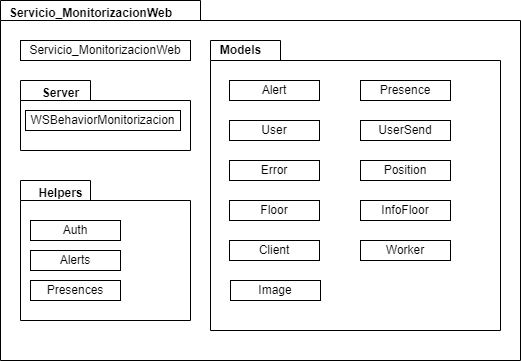
\includegraphics[width=12cm]{Imagenes/Diagrama-paquetes-backend}
    \caption{Diagrama de paquetes backend}
    \label{fig:paquetes-backend}
\end{figure}

Se observa como se tiene un módulo principal \textbf{Servicio\_MonitorizacionWeb} que es donde se procesa la llegada de eventos. Por otro lado se tiene el módulo \textbf{Server} donde se encuentra la lógica para recibir y enviar información a la aplicación web. Los módulos \textbf{Helpers} y \textbf{Models} son utilizados por los dos anteriores.\\




